% Options for packages loaded elsewhere
\PassOptionsToPackage{unicode}{hyperref}
\PassOptionsToPackage{hyphens}{url}
%
\documentclass[
  ignorenonframetext,
]{beamer}
\usepackage{pgfpages}
\setbeamertemplate{caption}[numbered]
\setbeamertemplate{caption label separator}{: }
\setbeamercolor{caption name}{fg=normal text.fg}
\beamertemplatenavigationsymbolsempty
% Prevent slide breaks in the middle of a paragraph
\widowpenalties 1 10000
\raggedbottom
\setbeamertemplate{part page}{
  \centering
  \begin{beamercolorbox}[sep=16pt,center]{part title}
    \usebeamerfont{part title}\insertpart\par
  \end{beamercolorbox}
}
\setbeamertemplate{section page}{
  \centering
  \begin{beamercolorbox}[sep=12pt,center]{part title}
    \usebeamerfont{section title}\insertsection\par
  \end{beamercolorbox}
}
\setbeamertemplate{subsection page}{
  \centering
  \begin{beamercolorbox}[sep=8pt,center]{part title}
    \usebeamerfont{subsection title}\insertsubsection\par
  \end{beamercolorbox}
}
\AtBeginPart{
  \frame{\partpage}
}
\AtBeginSection{
  \ifbibliography
  \else
    \frame{\sectionpage}
  \fi
}
\AtBeginSubsection{
  \frame{\subsectionpage}
}
\usepackage{amsmath,amssymb}
\usepackage{lmodern}
\usepackage{iftex}
\ifPDFTeX
  \usepackage[T1]{fontenc}
  \usepackage[utf8]{inputenc}
  \usepackage{textcomp} % provide euro and other symbols
\else % if luatex or xetex
  \usepackage{unicode-math}
  \defaultfontfeatures{Scale=MatchLowercase}
  \defaultfontfeatures[\rmfamily]{Ligatures=TeX,Scale=1}
\fi
\usetheme[]{Dresden}
\usecolortheme{whale}
% Use upquote if available, for straight quotes in verbatim environments
\IfFileExists{upquote.sty}{\usepackage{upquote}}{}
\IfFileExists{microtype.sty}{% use microtype if available
  \usepackage[]{microtype}
  \UseMicrotypeSet[protrusion]{basicmath} % disable protrusion for tt fonts
}{}
\makeatletter
\@ifundefined{KOMAClassName}{% if non-KOMA class
  \IfFileExists{parskip.sty}{%
    \usepackage{parskip}
  }{% else
    \setlength{\parindent}{0pt}
    \setlength{\parskip}{6pt plus 2pt minus 1pt}}
}{% if KOMA class
  \KOMAoptions{parskip=half}}
\makeatother
\usepackage{xcolor}
\IfFileExists{xurl.sty}{\usepackage{xurl}}{} % add URL line breaks if available
\IfFileExists{bookmark.sty}{\usepackage{bookmark}}{\usepackage{hyperref}}
\hypersetup{
  pdftitle={Identify Sustainable Credit Gap},
  pdfauthor={Nam Nguyen},
  hidelinks,
  pdfcreator={LaTeX via pandoc}}
\urlstyle{same} % disable monospaced font for URLs
\newif\ifbibliography
\setlength{\emergencystretch}{3em} % prevent overfull lines
\providecommand{\tightlist}{%
  \setlength{\itemsep}{0pt}\setlength{\parskip}{0pt}}
\setcounter{secnumdepth}{-\maxdimen} % remove section numbering
\PassOptionsToPackage{table}{xcolor}

\setbeamertemplate{caption}[numbered]

\setbeamertemplate{footline}{%
	\leavevmode%
	\hbox{\begin{beamercolorbox}[wd=.5\paperwidth,ht=2.5ex,dp=1.125ex,leftskip=.3cm plus1fill,rightskip=.3cm]{author in head/foot}%
			\usebeamerfont{author in head/foot}\insertshortauthor~(\insertshortinstitute)
		\end{beamercolorbox}%
		\begin{beamercolorbox}[wd=.5\paperwidth,ht=2.5ex,dp=1.125ex,leftskip=.3cm,rightskip=.3cm plus1fil]{title in head/foot}%
			\usebeamerfont{title in head/foot}\insertshorttitle\hfill\insertframenumber\,/\,\inserttotalframenumber
	\end{beamercolorbox}}%
	\vskip0pt%
}

\AtBeginSection{}
\AtBeginSubsection{}

\setbeamertemplate{section in toc}[sections numbered]
\setbeamertemplate{subsection in toc}[subsections numbered]

%\insertsectionnumber

\setbeamertemplate{itemize items}[circle]

\usepackage{amssymb,amsmath,amsfonts,eurosym,geometry,graphicx,caption,color,setspace,
	comment,footmisc,caption,pdflscape,array}
\usepackage{booktabs}   % for nice tables
\usepackage{multirow}
%\usepackage[round]{natbib}
\setbeamertemplate{caption}[numbered]
\usepackage[export]{adjustbox}

\usepackage[skip=1pt]{caption}
%\usepackage[capposition=top]{floatrow}

%\usepackage[caption = false]{subfig}
%\usepackage{floatrow}
\usepackage[capposition=bottom]{floatrow}

\usepackage{graphicx}
\usepackage{tabularx}
%\usepackage{threeparttable}
\usepackage{float}
\usepackage{mwe}
%\usepackage{subfig}
%\usepackage{polyglossia}
\usepackage{subcaption}
\setlength{\abovecaptionskip}{2pt}
%\usepackage[tight,TABTOPCAP]{subfigure}
\usepackage[round]{natbib}

\usepackage{multicol, latexsym, amsmath, amssymb}

\usepackage[normalem]{ulem}
\useunder{\uline}{\ul}{}
\usepackage{booktabs,caption}
\usepackage[flushleft]{threeparttable}

\usepackage{graphics}

\usepackage{longtable}

\usepackage{float}

\usepackage{amsbsy} %boldsymbol

%%in case of outdated TEX Live
\usepackage{lmodern}

\usepackage{appendixnumberbeamer}

%\graphicspath{{figures/}{../figures/}{D:/Presentations\figures/}}
\usepackage[normalem]{ulem}

\usepackage{siunitx}
\sisetup{
	round-mode          = places, % Rounds numbers
	round-precision     = 4, % to 2 places
}


\usepackage{graphicx} % Allows including images
\usepackage{booktabs} % Allows the use of \toprule, \midrule and \bottomrule in tables

\usepackage{arydshln} %can use hdashline


\PassOptionsToPackage{table}{xcolor}

\setbeamertemplate{caption}[numbered]

\setbeamertemplate{footline}{%
	\leavevmode%
	\hbox{\begin{beamercolorbox}[wd=.5\paperwidth,ht=2.5ex,dp=1.125ex,leftskip=.3cm plus1fill,rightskip=.3cm]{author in head/foot}%
			\usebeamerfont{author in head/foot}\insertshortauthor~(\insertshortinstitute)
		\end{beamercolorbox}%
		\begin{beamercolorbox}[wd=.5\paperwidth,ht=2.5ex,dp=1.125ex,leftskip=.3cm,rightskip=.3cm plus1fil]{title in head/foot}%
			\usebeamerfont{title in head/foot}\insertshorttitle\hfill\insertframenumber\,/\,\inserttotalframenumber
	\end{beamercolorbox}}%
	\vskip0pt%
}

%\AtBeginSection{}
\AtBeginSubsection{}

\setbeamertemplate{section in toc}[sections numbered]
\setbeamertemplate{subsection in toc}[subsections numbered]

%\insertsectionnumber

\setbeamertemplate{itemize items}[circle]

\usepackage{amssymb,amsmath,amsfonts,eurosym,geometry,graphicx,caption,color,setspace,
	comment,footmisc,caption,pdflscape,array}
\usepackage{booktabs}   % for nice tables
\usepackage{multirow}
%\usepackage[round]{natbib}
\setbeamertemplate{caption}[numbered]
\usepackage[export]{adjustbox}

\usepackage[skip=1pt]{caption}
%\usepackage[capposition=top]{floatrow}

%\usepackage[caption = false]{subfig}
%\usepackage{floatrow}
\usepackage[capposition=bottom]{floatrow}

\usepackage{graphicx}
\usepackage{tabularx}
%\usepackage{threeparttable}
\usepackage{float}
\usepackage{mwe}
%\usepackage{subfig}
%\usepackage{polyglossia}
\usepackage{subcaption}
\setlength{\abovecaptionskip}{2pt}
%\usepackage[tight,TABTOPCAP]{subfigure}
\usepackage[round]{natbib}

\usepackage{multicol, latexsym, amsmath, amssymb}

\usepackage[normalem]{ulem}
\useunder{\uline}{\ul}{}
\usepackage{booktabs,caption}
\usepackage[flushleft]{threeparttable}

\usepackage{graphics}

\usepackage{longtable}

\usepackage{float}

\usepackage{amsbsy} %boldsymbol

%%in case of outdated TEX Live
\usepackage{lmodern}

\usepackage{appendixnumberbeamer}

%\graphicspath{{figures/}{../figures/}{D:/Presentations\figures/}}
\usepackage[normalem]{ulem}

\usepackage{siunitx}
\sisetup{
	round-mode          = places, % Rounds numbers
	round-precision     = 4, % to 2 places
}


\usepackage{graphicx} % Allows including images
\usepackage{booktabs} % Allows the use of \toprule, \midrule and \bottomrule in tables

\usepackage{arydshln} %can use hdashline

\ifLuaTeX
  \usepackage{selnolig}  % disable illegal ligatures
\fi

\title{Identify Sustainable Credit Gap}
\author{Nam Nguyen}
\date{May 24, 2022}
\institute{UWM}

\begin{document}
\frame{\titlepage}

\hypertarget{introduction}{%
\section{Introduction}\label{introduction}}

\begin{frame}{Introduction}
\begin{block}{Introduction}
\protect\hypertarget{introduction-1}{}
\begin{itemize}
\tightlist
\item
  Motivation
\item
  Contribution
\item
  Literature Review
\end{itemize}
\end{block}

\begin{block}{Methodology}
\protect\hypertarget{methodology}{}
\begin{itemize}
\tightlist
\item
  Data
\item
  Empirical Model

  \begin{itemize}
  \tightlist
  \item
    Model Selection
  \item
    Model Averaging
  \item
    Weighted gap creation
  \end{itemize}
\end{itemize}
\end{block}

\begin{block}{Results}
\protect\hypertarget{results}{}
\end{block}
\end{frame}

\begin{frame}{Motivation}
\protect\hypertarget{motivation}{}
\begin{itemize}
\tightlist
\item
  To overcome model uncertainty in using credit gap as an early warning
  indicator (EWI) of systemic financial crises, we propose using model
  averaging of different credit gap measurements. The method is based on
  Bayesian Model Average - Raftery (1995)
\end{itemize}
\end{frame}

\begin{frame}{Motivation}
\protect\hypertarget{motivation-1}{}
\begin{itemize}
\tightlist
\item
  Area under the curve of operating characteristic (AUROC or AUC) has
  been widely used as a criterion to determine the performance of a EWI.
  But it has received some criticism regarding the lower left area of
  the curve representing low predictive ability of the indicator.
\item
  Borio and Drehmann (2009) and Beltran et al (2021) proposed a policy
  loss function constraining the relevance of the curve measurement to
  to just a portion where Type II error rate is less than 1/3 or at
  least 2/3 of the crises are predicted.\\
\item
  Detken (2014) proposed using partial standardized area under the curve
  (psAUC) as an alternative measurement of the performance of an EWI.
\end{itemize}
\end{frame}

\begin{frame}{Contribution}
\protect\hypertarget{contribution}{}
\begin{itemize}
\tightlist
\item
  Compare different credit gap measurements' performance as EWIs using a
  new criterion - partial standarized AUC (psAUC) contraining Type II
  error \textless{} 1/3.
\item
  Overcome model uncertainty by implementing model averaging. We
  incoporated psAUC values in the model selection and weighting process,
  instead of AUC or BIC values.
\item
  For ease of policy implication, we propose a single credit gap
  measurement from weighted averaging other popularly studied credit gap
  measurements.
\end{itemize}
\end{frame}

\begin{frame}{Literature Review}
\protect\hypertarget{literature-review}{}
Beltran (2021) - measured and the performance of BIS Basel credit gap,
Structural Time Series model (STM) gap, Moving average (MA) gap,
Hamilton filter gap, and optimized the smoothing parameters \(\rho\) in
those filters to minimize policy loss function.

\begin{align*}
L_{\theta,\rho}=\alpha TypeI(\theta)+(1-\alpha)TypeII(\theta)|TPR\ge2/3
\end{align*}

\begin{itemize}
\tightlist
\item
  \(\theta\) is the optimized threshold that minizes loss function.
\end{itemize}

Galán (2019) proposed rolling sample of 15 and 20 years when creating
one sided cycle.

Drehmann (2021) created Hamilton filter in a panel setting with fixed
coefficients on independent variable across countries.
\end{frame}

\begin{frame}{Data}
\protect\hypertarget{data}{}
Sample data periods:

\begin{itemize}
\tightlist
\item
  1970-Q4 - 2017-Q4 across 43 countries. We omit periods for countries
  with shorter credit measurement.
\end{itemize}

Systemic crisis data:

\begin{itemize}
\tightlist
\item
  European Systemic Risk Board crisis data set (Lo Duca et al.~2017)
\item
  Laeven and Valencia (2018)
\end{itemize}

Credit/GDP ratio data:

\begin{itemize}
\tightlist
\item
  Bank of International Settlement (BIS)

  \begin{itemize}
  \tightlist
  \item
    Latest Credit data is available at 2021:Q3
  \end{itemize}
\end{itemize}
\end{frame}

\hypertarget{model}{%
\section{Model}\label{model}}

\begin{frame}{Credit gaps creation}
\protect\hypertarget{credit-gaps-creation}{}
\begin{align}
    100*\frac{Credit}{GDP} &= y_t = \tau_{yt} + c_{yt}
\end{align}

\begin{itemize}
\tightlist
\item
  We created 90 candidate one-sided credit gap measurements based on the
  literature.

  \begin{itemize}
  \tightlist
  \item
    Once a country has more than 15 years of credit measurement
    available, we start storing its one-sided credit gap values onward.
  \end{itemize}
\end{itemize}
\end{frame}

\begin{frame}{Early Warning Indicator - Logistic regression:}
\protect\hypertarget{early-warning-indicator---logistic-regression}{}
\begin{align}
  pre.crisis_{ti} \sim credit.gap_{tij}
\end{align}

\begin{itemize}
\item
  \(i\) is country indicator. \(j\) is credit gap filter type
\item
  where \(pre.crisis_{it}=\) 1 or 0
\item
  The pre-crisis indicator is set to 1 when t is between 5-12 quarters
  before a systemic crisis.
\item
  We discard measurements between 1-4 quarters before a crisis, periods
  during a crisis and post-crisis periods identified in Lo Duca et
  al.~(2017) and Laeven and Valencia (2018).

  \begin{itemize}
  \tightlist
  \item
    The indicator is set to 0 at other periods.
  \item
    pre-crisis periods of imported crises identified in the dataset are
    also set to 0. However, we still discard measurements of periods
    during and post-crisis for imported crises.
  \end{itemize}
\end{itemize}
\end{frame}

\begin{frame}{AUROC}
\protect\hypertarget{auroc}{}
Each logistic regression with a different gap measurement yields a Area
Under Curve (AUC) of receiver operating characteristic value. There is
an underlying assumption that the higher the AUC value is the better
overall performance of a credit gap is as an EWI.

\begin{itemize}
\tightlist
\item
  However, the AUC value received some criticism regarding the area on
  its lower left corner, where the predictive power of the threshold
  (TPR) is low.
\end{itemize}

\begin{align*}
AUC = \int_0^1 TPR d(FPR)
\end{align*}

A ROC curve in the EWI setting represents True Positive Rate (TPR) and
False Positive Rate (FPR) of different credit gap thresholds indicating
a pre-crisis period. The thresholds are determined by the logistic
regression predicted probability values.
\end{frame}

\begin{frame}{partial standardised AUROC (psAUROC)}
\protect\hypertarget{partial-standardised-auroc-psauroc}{}
To overcome the issue of unnecessary information included in the full
AUC. An approach to estimate partial AUC was proposed.

Detken (2014) on partial standardized AUC:

\begin{quote}
``Instead of considering only the full AUROC (e.g.~Drehmann and
Juselius, 2014), this paper also presents a partial standardised AUROC
(psAUROC) that cuts off the area associated with a preference parameter
of \(\theta<0.5\).''\ldots{}
\end{quote}

\begin{quote}
``While the psAUROC has been used extensively in the area of medical
statistics to assess the performance of a classifier only in specific
regions of the ROC curve (e.g.~McClish, 1989 and Jiang et al., 1996), it
is a new approach in the literature evaluating EWMs''\ldots{}
\end{quote}

\begin{quote}
``The results reported in this paper show that the psAUROC can reveal
useful additional information as long as the partial area does not
become too restricted.''
\end{quote}
\end{frame}

\begin{frame}{pAUROC (or pAUC)}
\protect\hypertarget{pauroc-or-pauc}{}
Beltran (2021) constrainted the policy loss function to TPR \(\ge 2/3\)
or Type II error rate \(< 1/3\). They then estimated the policy loss
function value at different points on the ROC curve by assigning
different policy preferences \(\alpha\).

\(\Rightarrow\) In this paper, we propose to restrict the consideration
of the ROC curve to TPR \(\ge 2/3\), then estimate the psAUC of the
restricted ROC curve region instead. *Our notation of Type I and Type II
error follows Beltran (2021) which deviated from previous literature.

\begin{align}
pAUROC = \int_{\frac{2}{3}}^1 TNR \, d(TPR) = \int_{\frac{2}{3}}^1 specificity \, d(sensitivity)
\end{align}

\begin{itemize}
\tightlist
\item
  TNR = 1- FPR
\item
  FPR = Type I error rate, FNR = Type II error rate
\end{itemize}
\end{frame}

\begin{frame}{standardize psAUROC - Detken (2014)}
\protect\hypertarget{standardize-psauroc---detken-2014}{}
\begin{center}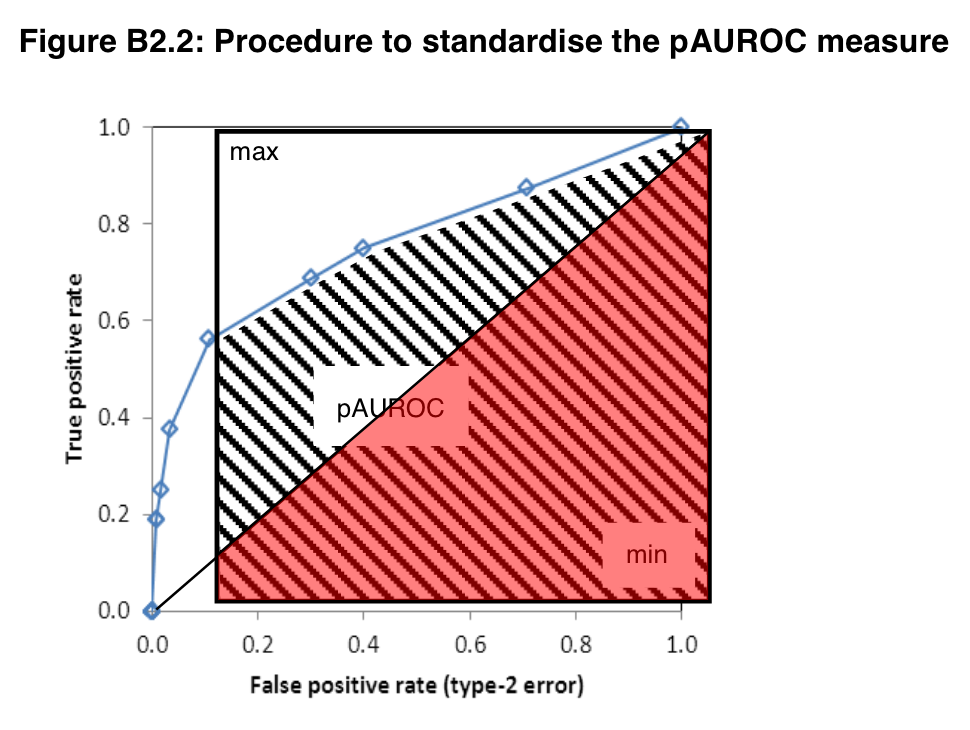
\includegraphics[width=0.7\linewidth]{Data/pAUC} \end{center}

\begin{align}
psAUROC = \frac{1}{2}\left[ 1+ \frac{pAUROC - min}{max - min}\right]
\end{align}
\end{frame}

\begin{frame}{Variable selection}
\protect\hypertarget{variable-selection}{}
\begin{block}{Comparing performance of individual credit gaps}
\protect\hypertarget{comparing-performance-of-individual-credit-gaps}{}
Using partial area under the curve (psAUC) values
\end{block}

\begin{block}{Test for gaps combination performance}
\protect\hypertarget{test-for-gaps-combination-performance}{}
Using Markov Chain Monte Carlo Model Comparison (\(MC^3\)) developed by
Madigan and York (1995). The method assigns posterior probability for
different credit gaps being selected in most likely models/combinations.
Babecky (2014) used this \(MC^3\) method to identify potential variables
in EWI models.

\begin{align*}
Model_k :  pre.crisis_{ti} \sim \sum\nolimits_j \beta_j * credit.gap_{tij}
\end{align*}
\end{block}

\begin{block}{Variable selection}
\protect\hypertarget{variable-selection-1}{}
We selected 29 credit gap measurements based on these 2 criteria.
\end{block}
\end{frame}

\begin{frame}{Variable selection (top 24 gaps ranked by psAUC)}
\protect\hypertarget{variable-selection-top-24-gaps-ranked-by-psauc}{}
\resizebox{\linewidth}{!}{
\begin{tabular}[t]{lrrr>{}rrrrr}
\toprule
Cycle & BIC & AIC & AUC & psAUC & c.Threshold & Type.I & Type.II & Policy.Loss.Function\\
\midrule
null & 0.0000 & 0.0000 & 0.5000 & \textbf{0.5000} & NA & 1.0000 & 0.0000 & 0.5000\\
c.bn620 & -108.0679 & -114.4506 & 0.7048 & \textbf{0.6379} & 0.6581 & 0.3962 & 0.3019 & 0.2481\\
c.hamilton28.panel & -149.8518 & -156.2346 & 0.7107 & \textbf{0.6359} & 9.7674 & 0.3912 & 0.3066 & 0.2470\\
c.hamilton13.panelr20 & -149.3378 & -155.7205 & 0.7030 & \textbf{0.6328} & 5.9924 & 0.4287 & 0.2547 & 0.2487\\
c.hamilton24.panel & -134.4093 & -140.7920 & 0.6991 & \textbf{0.6322} & 7.1794 & 0.4383 & 0.2689 & 0.2644\\
\addlinespace
c.hamilton13.panelr15 & -125.3568 & -131.7396 & 0.6923 & \textbf{0.6314} & 6.6651 & 0.4256 & 0.2925 & 0.2666\\
c.ma1 & -120.8108 & -127.1936 & 0.6922 & \textbf{0.6313} & 5.7812 & 0.3989 & 0.3160 & 0.2590\\
c.hamilton20.panelr15 & -134.3190 & -140.7017 & 0.6981 & \textbf{0.6311} & 7.5583 & 0.4612 & 0.2689 & 0.2850\\
c.hamilton20.panelr20 & -151.3035 & -157.6862 & 0.7045 & \textbf{0.6311} & 8.0087 & 0.4323 & 0.3066 & 0.2809\\
c.hamilton28.panelr20 & -164.6098 & -170.9925 & 0.7157 & \textbf{0.6300} & 10.8705 & 0.3946 & 0.2925 & 0.2412\\
\addlinespace
c.hamilton24.panelr20 & -155.8958 & -162.2786 & 0.7094 & \textbf{0.6299} & 9.2099 & 0.4253 & 0.2830 & 0.2610\\
c.hamilton24.panelr15 & -142.3051 & -148.6879 & 0.7027 & \textbf{0.6295} & 10.5773 & 0.3958 & 0.3160 & 0.2565\\
c.hamilton20.panel & -126.8625 & -133.2452 & 0.6907 & \textbf{0.6288} & 5.6212 & 0.4686 & 0.2830 & 0.2997\\
c.hamilton28.panelr15 & -153.5231 & -159.9058 & 0.7085 & \textbf{0.6267} & 11.5786 & 0.3871 & 0.3019 & 0.2410\\
c.hamilton13.panel & -133.9347 & -140.3175 & 0.6922 & \textbf{0.6250} & 4.9769 & 0.4285 & 0.2877 & 0.2664\\
\addlinespace
c.bn220 & -109.3128 & -115.6955 & 0.6963 & \textbf{0.6218} & 0.2776 & 0.4080 & 0.3255 & 0.2724\\
c.linear2 & -135.4069 & -141.7896 & 0.6879 & \textbf{0.6204} & 3.9989 & 0.4616 & 0.2925 & 0.2986\\
c.bn2 & -135.9914 & -142.3741 & 0.6842 & \textbf{0.6165} & 0.1864 & 0.4530 & 0.3113 & 0.3021\\
c.bn6 & -132.7915 & -139.1742 & 0.6835 & \textbf{0.6113} & 0.4710 & 0.4371 & 0.2830 & 0.2712\\
c.bn615 & -54.9953 & -61.3781 & 0.6756 & \textbf{0.6070} & 0.5680 & 0.4179 & 0.3255 & 0.2806\\
\addlinespace
c.bn215 & -83.9469 & -90.3297 & 0.6749 & \textbf{0.6047} & 0.1349 & 0.4761 & 0.3302 & 0.3357\\
c.poly420 & 3.5738 & -2.8090 & 0.5772 & \textbf{0.6011} & 0.1651 & 0.4980 & 0.3302 & 0.3570\\
BIS Basel gap & -121.5910 & -127.9738 & 0.6733 & \textbf{0.5960} & 3.0578 & 0.4441 & 0.3255 & 0.3032\\
c.bn4 & -169.1186 & -175.5014 & 0.6892 & \textbf{0.5943} & 1.2840 & 0.3837 & 0.3255 & 0.2532\\
c.bn415 & -89.6147 & -95.9975 & 0.6669 & \textbf{0.5929} & 0.4435 & 0.4792 & 0.2925 & 0.3152\\
\bottomrule
\end{tabular}}
\end{frame}

\hypertarget{model-averaging}{%
\section{Model averaging}\label{model-averaging}}

\begin{frame}{Bayesian Model Averging}
\protect\hypertarget{bayesian-model-averging}{}
The Bayesian Model Average method is formalized in Raftery (1995) to
account for model uncertainty.

\begin{block}{Model posterior probability}
\protect\hypertarget{model-posterior-probability}{}
equation (33): Model k posterior probability (weight): \begin{align}
  P(M_k|D) = \frac{P(D|M_k)P(M_k)}{\sum\nolimits_{l=1}^K P(D|M_l)P(M_l)} 
  \approx \frac{exp(-\frac{1}{2}BIC_k)}{\sum\nolimits_{l=1}^K exp(-\frac{1}{2}BIC_l)}
\end{align}

\begin{itemize}
\item
  Where \(P(M_k)\) is model prior probability and can be ignored if all
  models are assumed equal prior weights.
\item
  \(P(D|M_k)\) is marginal likehood. And
  \(P(D|M_k) \propto exp(-\frac{1}{2}BIC_k)\)
\item
  In which
  \(BIC_k = 2log (Bayesfactor_{sk}) = \chi^2_{sk} - df_klog(n)\). s
  indicates the saturated model.
\end{itemize}
\end{block}
\end{frame}

\begin{frame}{Model posterior probability}
\protect\hypertarget{model-posterior-probability-1}{}
\begin{itemize}
\tightlist
\item
  \(BIC_k = 2log (Bayesfactor_{sk}) = \chi^2_{sk} - df_klog(n)\)
\item
  \(\chi^2_{sk}\) is the deviance of model K from the the saturated
  model

  \begin{itemize}
  \tightlist
  \item
    \(\chi^2_{sk} = 2(ll(Ms) - ll(Mk))\)
  \item
    \(ll(Mk)\) is the log-likelihood of model Mk given data D
  \end{itemize}
\end{itemize}

\begin{block}{Alternate deviance measurement}
\protect\hypertarget{alternate-deviance-measurement}{}
We propose using psAUC instead of log-likelihood in the measurement of
deviance. Hence, an alternative BIC value can be estimated at:

\begin{align}
BIC_{alt,k} &= 2log (Bayesfactor_{alt,sk}) \\
&= 2(1000*(psAUC_s-psAUC_k)) - df_klog(n)
\end{align} - We scaled the psAUC value by 1000 since \(0<psAUC<1\).
Also, by design, \(psAUC_s=1\).
\end{block}
\end{frame}

\begin{frame}{Posterior distribution of coefficients of interest:}
\protect\hypertarget{posterior-distribution-of-coefficients-of-interest}{}
\(\beta_j\) is the coefficient of credit gap j (\(c_j\)) in a logistic
regression model k against pre-crisis indicator. When considering a
particular \(\beta_1\) :

\begin{align*}
p(\beta_1|D, \beta_1\ne 0) = \sum\nolimits_{A_1} p(\beta_1|D,M_k)p'(M_k|D)
\end{align*}

\begin{itemize}
\tightlist
\item
  where \(p'(M_k|D)=p(M_k|D)/ pr[\beta_1 \ne 0|D]\)
\item
  and \(pr[\beta_1 \ne 0|D] = \sum\limits_{A_1} P(M_k|D)\)

  \begin{itemize}
  \tightlist
  \item
    this is the probability that \(\beta_1\) is in the averaged model
  \item
    \(A_1= \{M_k: k=1,...,K; \beta_1 \ne 0\}\), is the set of models
    that includes \(\beta_1\)
  \end{itemize}
\end{itemize}
\end{frame}

\begin{frame}{Approximation of Bayesian point estimate:}
\protect\hypertarget{approximation-of-bayesian-point-estimate}{}
\begin{align}
\hat{\beta}_1 = E[\beta_1|D, \beta_1\ne 0] = \sum\limits_{A_1} \hat{\beta}_1(k)p'(M_k|D)
\end{align}

\(SD^2[\beta_1|D, \beta_1\ne 0] =[\sum\limits_{A_1}[se_1^2(k)+]+\hat{\beta_1}(k)]p'(M_k|D) - E[\beta_1|D, \beta_1\ne 0]^2\)

\begin{itemize}
\tightlist
\item
  Where \(\hat{\beta}_1(k)\) and \(se_1^2(k)\) are respectively the MLE
  and standard error of \(\beta_1\) under the model \(M_k\). (Leamer
  1978, p.118; Raftery 1993a)
\end{itemize}
\end{frame}

\hypertarget{weighted-credit-gap-creation}{%
\section{Weighted credit gap
creation}\label{weighted-credit-gap-creation}}

\begin{frame}{Weighted averaged credit gap - motivation}
\protect\hypertarget{weighted-averaged-credit-gap---motivation}{}
GLM binomial estimation: \begin{align*}
\widehat{pre.crisis}_{ti} = \widehat{probability}_{ti} = \frac {1}{1+exp(-(a+\sum\nolimits_j \hat{\beta}_j c_{tij}))}
\end{align*}

\begin{itemize}
\tightlist
\item
  With \(\hat{\beta}_j\) =
  \(E[\beta_j|D, \beta_j\ne 0] = \sum\limits_{A_j} \hat{\beta}_j(k)p'(M_k|D)\)
\end{itemize}

\(\Rightarrow\) We propose a single weighted credit gap \(\hat{c}_{ti}\)
that satisfies: \begin{align*}
\frac {1}{1+exp(-(a+\hat{\beta} \hat{c}_{ti}))}= \frac {1}{1+exp(-(a+\sum\nolimits_j \hat{\beta}_j c_{tij}))} \\
\end{align*} OR \begin{align}
\sum\limits_j \hat{\beta}_j c_{tij} = \hat{\beta} \hat{c}_{ti}
\end{align}
\end{frame}

\begin{frame}{Weighted averaged credit gap - creation}
\protect\hypertarget{weighted-averaged-credit-gap---creation}{}
\begin{align*}
\sum\limits_j \hat{\beta}_j c_{tij} = \hat{\beta} \hat{c}_{ti}
\end{align*}

We then propose \(\hat{\beta} = \sum\nolimits_j \hat{\beta}_j\)

Therefore,

\begin{align}
\hat{c}_{ti} = \frac{\sum\nolimits_j (\hat{\beta}_j c_{tij})}{\sum\nolimits_j\hat{\beta}_j} = \sum\nolimits_j w_j c_{tij}
\end{align}

The weight of each candidate credit gap j is
\(w_j = \frac{\hat{\beta}_j}{\sum\nolimits_j\hat{\beta}_j}\)
\end{frame}

\begin{frame}{One-sided crisis weighted averaged credit gap}
\protect\hypertarget{one-sided-crisis-weighted-averaged-credit-gap}{}
\begin{itemize}
\item
  The weight of each candidate credit gap j is
  \(w_j = \frac{\hat{\beta}_j}{\sum\nolimits_j\hat{\beta}_j}\)
\item
  We save the weights \(w_j\) at every incremental period \(t\) of
  available data to create a one-sided weight vector \(w_{tj}\).
\end{itemize}

\(\Rightarrow\) To create one-sided crisis weighted averaged credit gap
for each country \(i\) (\(\hat{c}_{ti}\)), we compute: \begin{align}
\hat{c}_{ti,one-sided} = \sum\nolimits_{j} w_{tj} * c_{tij}
\end{align}
\end{frame}

\hypertarget{empirical-results}{%
\section{Empirical Results}\label{empirical-results}}

\begin{frame}{Comparing performance of weighted gap as an EWI}
\protect\hypertarget{comparing-performance-of-weighted-gap-as-an-ewi}{}
\resizebox{\linewidth}{!}{
\begin{tabular}[t]{llrrr>{}rrrrr}
\toprule
  & Cycle & BIC & AIC & AUC & psAUC & c.Threshold & Type.I & Type.II & Policy.Loss.Function\\
\midrule
1 & null & 0.0000 & 0.0000 & 0.5000 & \textbf{0.5000} & NA & 1.0000 & 0.0000 & 0.5000\\
\textbf{2} & \textbf{1-sided weighted-gap} & \textbf{-187.2874} & \textbf{-193.6701} & \textbf{0.7407} & \textbf{\textbf{0.6809}} & \textbf{1.5478} & \textbf{0.3724} & \textbf{0.2877} & \textbf{0.2215}\\
3 & c.bn620 & -108.0679 & -114.4506 & 0.7048 & \textbf{0.6379} & 0.6581 & 0.3962 & 0.3019 & 0.2481\\
4 & c.hamilton28.panel & -149.8518 & -156.2346 & 0.7107 & \textbf{0.6359} & 9.7674 & 0.3912 & 0.3066 & 0.2470\\
5 & c.hamilton13.panelr20 & -149.3378 & -155.7205 & 0.7030 & \textbf{0.6328} & 5.9924 & 0.4287 & 0.2547 & 0.2487\\
\addlinespace
6 & c.hamilton24.panel & -134.4093 & -140.7920 & 0.6991 & \textbf{0.6322} & 7.1794 & 0.4383 & 0.2689 & 0.2644\\
7 & c.hamilton13.panelr15 & -125.3568 & -131.7396 & 0.6923 & \textbf{0.6314} & 6.6651 & 0.4256 & 0.2925 & 0.2666\\
8 & c.ma1 & -120.8108 & -127.1936 & 0.6922 & \textbf{0.6313} & 5.7812 & 0.3989 & 0.3160 & 0.2590\\
9 & c.hamilton20.panelr15 & -134.3190 & -140.7017 & 0.6981 & \textbf{0.6311} & 7.5583 & 0.4612 & 0.2689 & 0.2850\\
10 & c.hamilton20.panelr20 & -151.3035 & -157.6862 & 0.7045 & \textbf{0.6311} & 8.0087 & 0.4323 & 0.3066 & 0.2809\\
\addlinespace
11 & c.hamilton28.panelr20 & -164.6098 & -170.9925 & 0.7157 & \textbf{0.6300} & 10.8705 & 0.3946 & 0.2925 & 0.2412\\
12 & c.hamilton24.panelr20 & -155.8958 & -162.2786 & 0.7094 & \textbf{0.6299} & 9.2099 & 0.4253 & 0.2830 & 0.2610\\
18 & c.linear2 & -135.4069 & -141.7896 & 0.6879 & \textbf{0.6204} & 3.9989 & 0.4616 & 0.2925 & 0.2986\\
19 & c.bn2 & -135.9914 & -142.3741 & 0.6842 & \textbf{0.6165} & 0.1864 & 0.4530 & 0.3113 & 0.3021\\
20 & c.bn6 & -132.7915 & -139.1742 & 0.6835 & \textbf{0.6113} & 0.4710 & 0.4371 & 0.2830 & 0.2712\\
\addlinespace
21 & c.bn615 & -54.9953 & -61.3781 & 0.6756 & \textbf{0.6070} & 0.5680 & 0.4179 & 0.3255 & 0.2806\\
22 & c.bn215 & -83.9469 & -90.3297 & 0.6749 & \textbf{0.6047} & 0.1349 & 0.4761 & 0.3302 & 0.3357\\
23 & c.poly420 & 3.5738 & -2.8090 & 0.5772 & \textbf{0.6011} & 0.1651 & 0.4980 & 0.3302 & 0.3570\\
\textbf{24} & \textbf{BIS Basel gap} & \textbf{-121.5910} & \textbf{-127.9738} & \textbf{0.6733} & \textbf{\textbf{0.5960}} & \textbf{3.0578} & \textbf{0.4441} & \textbf{0.3255} & \textbf{0.3032}\\
25 & c.bn4 & -169.1186 & -175.5014 & 0.6892 & \textbf{0.5943} & 1.2840 & 0.3837 & 0.3255 & 0.2532\\
\addlinespace
26 & c.bn415 & -89.6147 & -95.9975 & 0.6669 & \textbf{0.5929} & 0.4435 & 0.4792 & 0.2925 & 0.3152\\
27 & c.bn520 & -99.7674 & -106.1501 & 0.6744 & \textbf{0.5928} & 0.5016 & 0.4234 & 0.3302 & 0.2883\\
28 & c.stm15 & -79.5531 & -85.9358 & 0.6575 & \textbf{0.5924} & 2.0027 & 0.4778 & 0.3160 & 0.3281\\
29 & c.hp125k1 & -92.2897 & -98.6725 & 0.6562 & \textbf{0.5924} & 2.5216 & 0.4547 & 0.3302 & 0.3158\\
30 & c.hp221k1 & -106.8842 & -113.2669 & 0.6656 & \textbf{0.5921} & 2.6641 & 0.4561 & 0.3160 & 0.3079\\
\bottomrule
\end{tabular}}
\end{frame}

\begin{frame}{Plot weighted gap against BIS gap}
\protect\hypertarget{plot-weighted-gap-against-bis-gap}{}
\begin{center}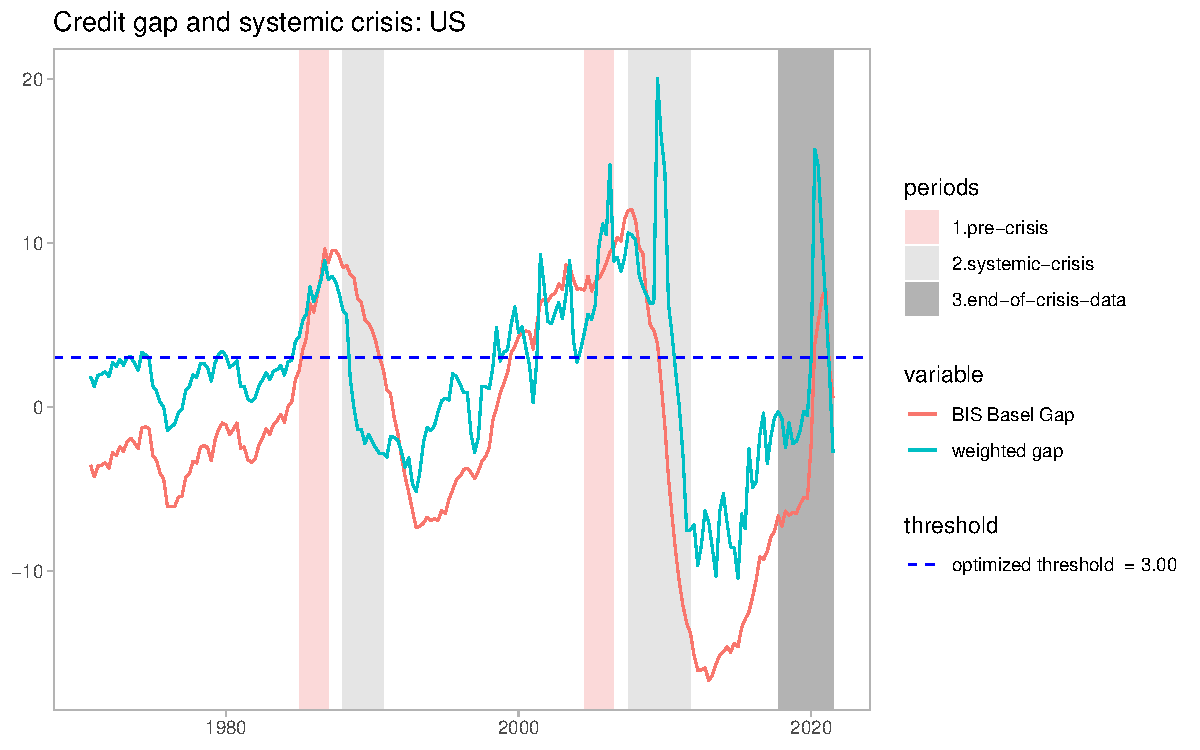
\includegraphics[width=1\linewidth]{../Data/Output/Graphs/Weighted_credit_gap_US} \end{center}
\end{frame}

\begin{frame}{Plot weighted gap against BIS gap}
\protect\hypertarget{plot-weighted-gap-against-bis-gap-1}{}
\begin{center}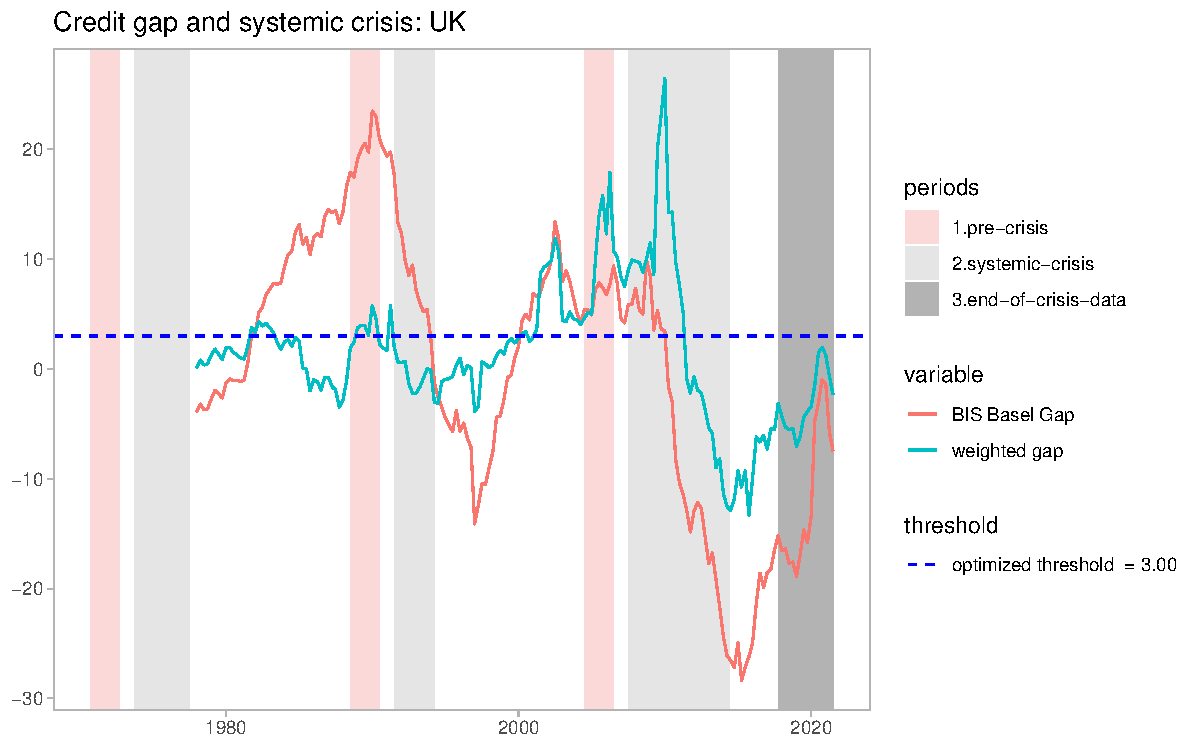
\includegraphics[width=1\linewidth]{../Data/Output/Graphs/Weighted_credit_gap_UK} \end{center}
\end{frame}

\end{document}
